\chapter{Hierarchical Models}
Hierarchical model is useful in the sense that it allows between-group information sharing. In contrast, for frequentists, two groups of sample are usually assumed to be drawn from different distributions. A direct result is that the estimation on the average is not a continuum but discrete
\begin{equation*}
    \hat{\theta}_i = 
    \begin{cases}
        \bar{y_i} & \text{if } \mu_1 \neq \mu_2, \\
        \frac{\sum Y_{i1} + \sum Y_{i2}}{n_1 + n_2} & \text{if } \mu_1 = \mu_2.
    \end{cases}
\end{equation*}
An even worse disturbance is that we are only using within-group data, potentially making our estimation less robust. To save the world, the hierarchical Bayesian model is come to the rescue. We start with a simple 2-group case. For simplicity, we will only talk about 1-dimensional distributions.

\section{Two-Group Hierarchy}
Bayesians model the two groups as follow:
\begin{align*}
    Y_{i, 1} &= \mu + \delta + \epsilon_{i, 1} \\
    Y_{i, 2} &= \mu - \delta + \epsilon_{i, 2} \\
    \{\epsilon_{i,j}\} &\sim_{iid} N(0, \sigma^2)
\end{align*}
where the three parameters follows $p(\mu, \delta, \sigma^2) = p(\mu) \times p(\delta) \times p(\sigma^2)$ with
\begin{align*}
    \mu &\sim N(\mu_0, \gamma_0^2) \\
    \delta &\sim N(\delta_0, \tau_0^2) \\
    \sigma^2 \sim& InvGamma(\nu_0/2, \nu_0\sigma_0^2/2)
\end{align*}

\subsection*{Full Conditional}
\begin{equation*}
    \mu | \vec{Y_1}, \vec{Y_2}, \delta, \sigma^2 \sim N(\mu_n, \gamma_n^2)
\end{equation*}
\begin{equation*}
    \delta | \vec{Y_1}, \vec{Y_2}, \mu, \sigma^2 \sim N(\delta_n, \tau_n^2)
\end{equation*}
\begin{equation*}
    \sigma^2 | \vec{Y_1}, \vec{Y_2}, \delta, \mu \sim InvGamma(\nu_n/2, \nu_n\sigma_n^2/2)
\end{equation*}

\subsection*{Model Structure Outline}
\begin{figure}[H]
    \centering
    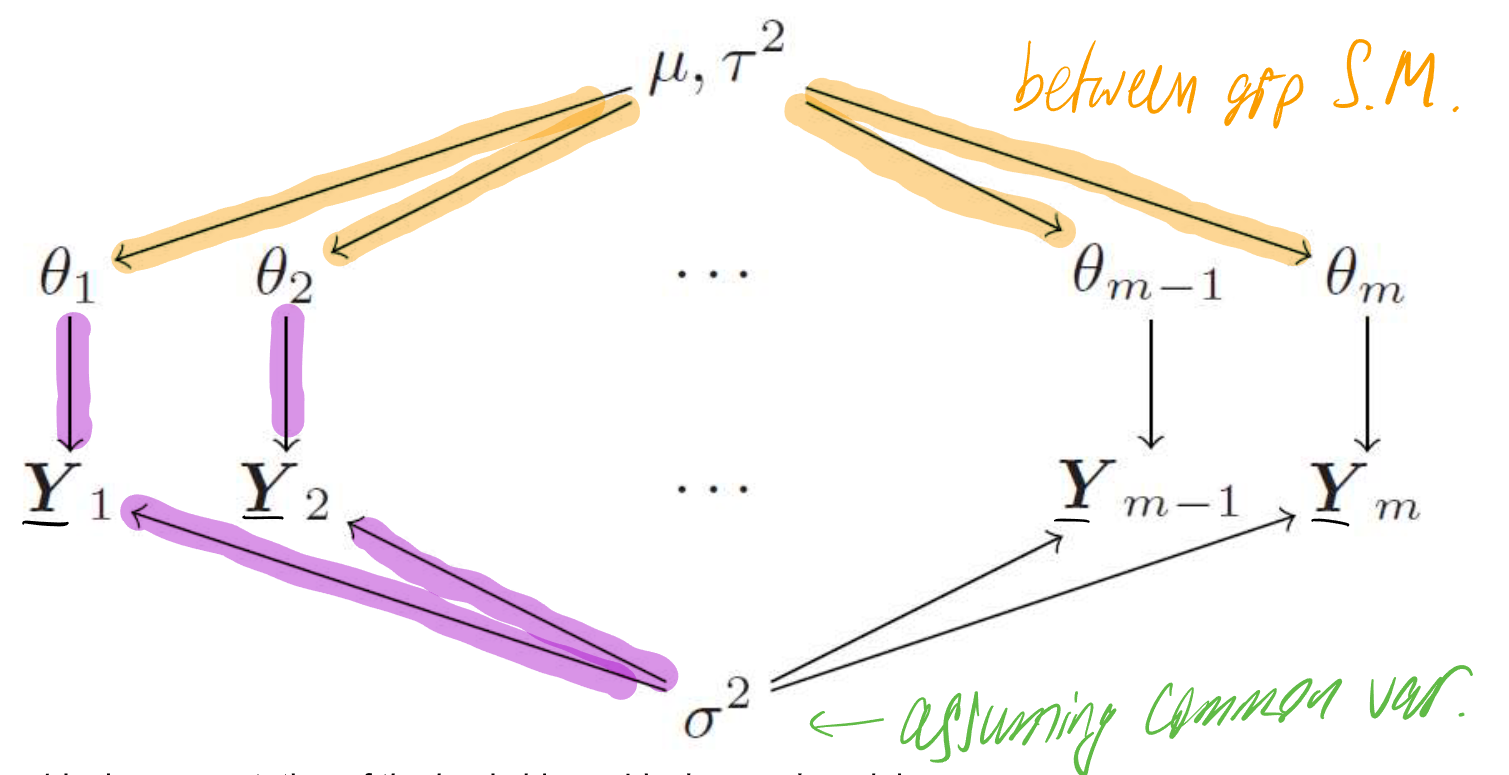
\includegraphics[width=0.9\textwidth]{~/Documents/Lecture_Notes/2024_FALL_JHU/Bayesian_Statistics/Figures/Hierarchical_Bayesian_Models.png}
\end{figure}

\section{Multigroup Hierarchy}

\subsection*{Prior}
\begin{equation*}
    \sigma^2 \sim InvGamma(\nu_0/2, \nu_0\sigma_0^2/2)
\end{equation*}
\begin{equation*}
    \tau^2 \sim InvGamma(\eta_0/2, \eta_0\tau_0^2/2)
\end{equation*}
\begin{equation*}
    \mu \sim N(\mu_0, \gamma_0^2)
\end{equation*}

\subsection*{Full Conditional Distribution}
We can use the following results to estimate the parameters. 
\begin{equation*}
    \mu | \theta_1, \ldots, \theta_m, \tau^2 \sim N(\frac{m\bar{\theta}/\tau^2 + \mu_0/\gamma_0^2}{m/\tau^2 + 1/\gamma_0^2}, [m/\tau^2 + 1/\gamma_0^2]^{-1})
\end{equation*}
\begin{equation*}
    \tau^2 | \vec{\theta}, \mu \sim InvGamma(\frac{\eta_0 + m}{2}, \frac{\eta_0\tau_0^2 + \sum_{i=1}^{m}(\theta_i - \mu)^2}{2})
\end{equation*}
\begin{equation*}
    \theta_j | \vec{Y_j}, \sigma^2 \sim N(\frac{n_j\bar{y}_j/\sigma^2 + \mu/\tau^2}{n_j/\sigma^2 + 1/\tau^2}, [n_j/\sigma^2 + 1/\tau^2]^{-1})
\end{equation*}
\begin{equation*}
    \sigma^2 | \theta, \vec{Y} \sim InvGamma(\frac{1}{2}\big[\nu_0 + \sum_{j=1}^{m}n_j\big], \frac{1}{2}\big[\nu_0\sigma_0^2 + \sum_{j=1}^{m}\sum_{i=1}^{n_j}(Y_{i,j} - \theta_j)^2\big])
\end{equation*}
